\documentclass[11pt]{article}
\usepackage{mathblatt}
% gesetzt von werkzeuge/setzer.py (Sorte selbst) aus dem Lernweg BGG
% und den Bankzeilen; Muster bau/proben/2026-10-09/hypotenuse-muster.
\usepackage{enumitem}
\usepackage{adjustbox,varwidth}
\newgeometry{a4paper,margin=18mm,top=15mm,bottom=20mm,footskip=9mm}
\pagestyle{fancy}\fancyhf{}\renewcommand{\headrulewidth}{0pt}
\fancyfoot[L]{\footnotesize\color{mbgrau}BGG \textperiodcentered{} Terme aufstellen}
\fancyfoot[R]{\footnotesize\color{mbgrau}\thepage}
\setlength{\parskip}{3pt}
\renewcommand{\kreuz}[1]{\mbox{$\square$\ #1}\quad}
\newcommand{\kreuzl}[1]{\par\hangindent1.4em\hangafter1\noindent$\square$\ #1}
\newcommand{\aufg}[3]{\par\noindent\makebox[0pt][r]{#3}\begin{minipage}[t]{\linewidth}#1\end{minipage}\par}
\newcommand{\aufgg}[4]{\par\noindent\makebox[0pt][r]{#4}\begin{minipage}[t]{0.6\linewidth}\vspace{0pt}#1\end{minipage}\hfill
  \begin{minipage}[t]{0.37\linewidth}\vspace{0pt}\centering #2\end{minipage}\par}
\newcommand{\nr}[1]{\makebox[7mm][l]{\textbf{#1}}}
\newcommand{\lsg}[3]{\par\noindent\begin{minipage}[t]{9mm}\textbf{#1}\end{minipage}%
  \begin{minipage}[t]{52mm}\raggedright\bfseries\boldmath #2\end{minipage}\hspace{3mm}%
  \begin{minipage}[t]{\dimexpr\linewidth-64mm\relax}\raggedright\small #3\end{minipage}\par\vspace{4pt}}
\newlength{\kr}
\makeatletter
\newcommand{\karomerk}[2]{\protected@write\@auxout{}{\string\karoseite{#1}{#2}{\thepage}}}
\newcommand{\karoseite}[3]{\expandafter\xdef\csname karo@#1@#2\endcsname{#3}}
\newcommand{\karohinweis}[3]{\karomerk{h}{#1}\ifcsname karo@k@#1\endcsname
  \ifnum\csname karo@k@#1\endcsname=0\csname karo@h@#1\endcsname\relax#2\else#3\fi
  \else#3\fi}
\makeatother
\begin{document}

\noindent{\LARGE\bfseries Terme aufstellen}\par\smallskip
\noindent{\small\color{mbgrau}Selbstlernheft Klasse 7 \textperiodcentered{} mit Lösungsheft \textperiodcentered{} Kennung BGG}\par\medskip
\noindent\textbf{So nutzt du das Heft:} Lies im Abschnitt das Beispiel. Rechne dann die Aufgaben der Reihe nach und vergleiche jede sofort mit dem Lösungsheft. Kreuze „kann ich“ an, wenn du die letzte Aufgabe (\emph{Ziel}) allein schaffst.\par
\noindent Mehr Aufgaben zu einem Abschnitt: Kennung deinem Nachhilfelehrer schicken (z.\,B. „BGG mehr B“).\par\medskip
{\arrayrulecolor{mbgrau}\renewcommand{\arraystretch}{1.3}
\noindent\begin{tabular}{|>{\bfseries}p{10mm}|p{112mm}|>{\raggedleft\arraybackslash}p{10mm}|>{\centering\arraybackslash}p{14mm}|}\hline
\rowcolor{black!8} & \textbf{Abschnitt} & \textbf{Seite} & \textbf{kann ich}\\\hline
A & Rechenwörter in Terme übersetzen & \pageref{s:A} & $\square$\\\hline
B & Klammer, wenn ein Ergebnis weiterverarbeitet wird & \pageref{s:B} & $\square$\\\hline
C & Term zur Figur: Umfang und Flächeninhalt & \pageref{s:C} & $\square$\\\hline
D & Terme in Sachaufgaben & \pageref{s:D} & $\square$\\\hline
T & Probetest & \pageref{s:T} & $\square$\\\hline
\end{tabular}}\par\bigskip

\begin{tcolorbox}[colback=mbkasten,colframe=mbgrau,boxrule=0.5pt,arc=1mm,left=3mm,right=3mm,top=2mm,bottom=2mm,title={\bfseries Formel auf einen Blick},coltitle=black,colbacktitle=black!10]
{\Large Variable festlegen $\to$ Stück für Stück übersetzen $\to$ Klammer, wenn ein Ergebnis weiterverarbeitet wird $\to$ Probe mit einer Zahl}\par\medskip
In Worten: Ein Term ist eine Rechnung mit einer Variablen. Setzt du eine Zahl ein, muss dasselbe herauskommen wie beim Rechnen nach dem Text.\par\medskip
\end{tcolorbox}
\medskip\noindent\textbf{Typische Fehler – so nicht}\par\smallskip
\noindent\nr{$\times$}Ein Term ist kein Ergebnis: $3x + 4$ bleibt so stehen, es ist nicht $7x$.\par
\clearpage\label{s:A}\noindent\colorbox{black!12}{\makebox[10mm]{\Large\bfseries\strut A}}\hspace{3mm}{\Large\bfseries Rechenwörter in Terme übersetzen}\par\smallskip
\noindent Übersetze Stück für Stück in der Reihenfolge, in der gerechnet wird: Was zuerst mit $x$ geschieht, schreibst du zuerst.\par\medskip
\noindent\textbf{Formel}\par\nopagebreak\noindent\hspace*{4mm}\begin{minipage}{\dimexpr\linewidth-4mm\relax}das Dreifache von $x$: $3x$ \quad die Hälfte von $x$: $x : 2$ \quad das Produkt aus 3 und $x$: $3 \cdot x = 3x$ \par\vspace{3pt} $x$ um 4 vergrößert: $x + 4$ \quad $x$ um 4 vermindert: $x - 4$ \quad aber 4 vermindert um $x$: $4 - x$ \par\vspace{3pt} 4 mehr als $x$: $x + 4$ \quad 4 weniger als $x$: $x - 4$ \quad dreimal so viel wie $x$: $3x$\end{minipage}\par\medskip
\noindent\textbf{Beispiel}\quad Das Doppelte einer Zahl $x$ wird um 7 vermindert. Schreibe dazu einen Term.\par\smallskip
\noindent\par\noindent\hangindent6mm\hangafter1\makebox[6mm][l]{\textbf{1}}Was geschieht zuerst mit $x$? Es wird verdoppelt: \quad $2x$\par\smallskip\par\noindent\hangindent6mm\hangafter1\makebox[6mm][l]{\textbf{2}}„um 7 vermindert“ heißt minus 7, hinten angehängt: \quad $2x - 7$\par\smallskip\par\noindent\hangindent6mm\hangafter1\makebox[6mm][l]{\textbf{3}}Probe mit einer Zahl, z.\,B. $x = 5$: Das Doppelte ist $10$, um 7 vermindert $3$. \ Term: $2 \cdot 5 - 7 = 3$. Passt.\par\smallskip\par\medskip
\noindent\textbf{Aufgaben}\hspace{1em}{\small\color{mbgrau}\karohinweis{A}{Rechne unten im Karo.}{Rechne auf einem extra Blatt.} Vergleiche jede Aufgabe gleich mit dem Lösungsheft.}\par\smallskip
\aufg{\hangindent7mm\hangafter1\nr{1.}Schreibe als Term. \par\vspace{3pt} a)~das Fünffache von $x$ \qquad b)~$x$ um 8 vergrößert \qquad c)~$x$ um 6 vermindert \par\vspace{3pt} d)~die Hälfte von $x$ \qquad e)~10 vermindert um $x$ \qquad f)~das Produkt aus 7 und $x$}{}{}
\medskip
\aufg{\hangindent7mm\hangafter1\nr{2.}Das Siebenfache einer Zahl $x$ wird um 3 vermindert. Kreuze den passenden Term an.\par\smallskip\leftskip7mm \kreuz{$7 \cdot (x - 3)$}\ \kreuz{$3 - 7x$}\par\kreuz{$7x - 3$}\ \kreuz{$7x - 3x$}}{}{}
\medskip
\aufg{\hangindent7mm\hangafter1\nr{3.}Schreibe als Term. \par\vspace{3pt} a)~Das Dreifache einer Zahl $x$ wird um 4 vergrößert. \par b)~Das Vierfache von $x$ wird um 9 vermindert. \par c)~20 wird um das Doppelte von $x$ vermindert. \par d)~Die Hälfte von $x$ wird um 1 vergrößert.}{}{}
\medskip
\aufg{\hangindent7mm\hangafter1\nr{4.}Lena ist $x$ Jahre alt. Ihr Bruder Tim ist 4 Jahre älter als Lena. Ihre Mutter ist dreimal so alt wie Lena. \par a)~Schreibe je einen Term für das Alter von Tim und von der Mutter. \par b)~Lena ist 12 Jahre alt. Ist die Mutter älter als 35 Jahre?}{}{{\scriptsize\color{mbgrau}Ziel\hspace{2mm}}}
\medskip
\par\vspace{3mm}\setlength{\kr}{\dimexpr\pagegoal-\pagetotal-10mm\relax}%
\ifdim\kr>12mm\karomerk{k}{A}\noindent{\scriptsize\color{mbgrau}Platz zum Rechnen}\par\nointerlineskip\vspace{1mm}\noindent
\begin{tikzpicture}\clip (0,0) rectangle ({\linewidth-0.5mm},\kr);\draw[black!16,line width=0.3pt,step=5mm] (0,0) grid (\linewidth,\kr);\end{tikzpicture}\fi\par
\clearpage\label{s:B}\noindent\colorbox{black!12}{\makebox[10mm]{\Large\bfseries\strut B}}\hspace{3mm}{\Large\bfseries Klammer, wenn ein Ergebnis weiterverarbeitet wird}\par\smallskip
\noindent Wird eine Summe oder Differenz als Ganzes weiterverarbeitet (verdoppelt, halbiert, mit einer Zahl malgenommen), kommt sie in Klammern.\par\medskip
\noindent\textbf{Formel}\par\nopagebreak\noindent\hspace*{4mm}\begin{minipage}{\dimexpr\linewidth-4mm\relax}Die Summe aus $x$ und 3 wird verdoppelt: $2 \cdot (x + 3)$ \par aber: Das Doppelte von $x$ wird um 3 vergrößert: $2x + 3$ \par\vspace{3pt} Die Summe aus $x$ und 6 wird halbiert: $(x + 6) : 2$ \par\vspace{3pt} 3 Personen zahlen je $x + 2$ Euro: $3 \cdot (x + 2)$\end{minipage}\par\medskip
\noindent\textbf{Beispiel}\quad Die Differenz aus dem Vierfachen einer Zahl $x$ und 3 wird verdoppelt. Schreibe dazu einen Term.\par\smallskip
\noindent\par\noindent\hangindent6mm\hangafter1\makebox[6mm][l]{\textbf{1}}Das Vierfache von $x$: \quad $4x$\par\smallskip\par\noindent\hangindent6mm\hangafter1\makebox[6mm][l]{\textbf{2}}Die Differenz aus $4x$ und 3: \quad $4x - 3$\par\smallskip\par\noindent\hangindent6mm\hangafter1\makebox[6mm][l]{\textbf{3}}Diese Differenz wird verdoppelt – als Ganzes, also in Klammern: \quad $2 \cdot (4x - 3)$\par\smallskip\par\noindent\hangindent6mm\hangafter1\makebox[6mm][l]{\textbf{4}}Probe mit $x = 2$: Vierfaches $8$, minus 3 ergibt $5$, verdoppelt $10$. \ Term: $2 \cdot (4 \cdot 2 - 3) = 2 \cdot 5 = 10$. Passt.\par\smallskip\par\medskip
\noindent\textbf{Aufgaben}\hspace{1em}{\small\color{mbgrau}\karohinweis{B}{Rechne unten im Karo.}{Rechne auf einem extra Blatt.} Vergleiche jede Aufgabe gleich mit dem Lösungsheft.}\par\smallskip
\aufg{\hangindent7mm\hangafter1\nr{1.}Schreibe als Term. \par a)~Die Summe aus $x$ und 5 wird verdreifacht. \par b)~Die Differenz aus $x$ und 2 wird mit 4 multipliziert. \par c)~Die Summe aus $x$ und 8 wird halbiert.}{}{}
\medskip
\aufg{\hangindent7mm\hangafter1\nr{2.}Schreibe als Term. Nicht jeder braucht eine Klammer. \par a)~Verdopple eine Zahl $x$, addiere 5 und verdreifache das Ergebnis. \par b)~Die Summe aus dem Dreifachen von $x$ und 4 wird halbiert. \par c)~Vervierfache eine Zahl $x$ und addiere dann 6.}{}{}
\medskip
\aufg{\hangindent7mm\hangafter1\nr{3.}Die Differenz aus dem Fünffachen einer Zahl $x$ und 4 wird verdreifacht. Kreuze den passenden Term an.\par\smallskip\leftskip7mm \kreuz{$(5x - 4) : 3$}\ \kreuz{$5x : 4 \cdot 3$}\par\kreuz{$3 \cdot (5x - 4)$}\ \kreuz{$5x - 4 \cdot 3$}}{}{}
\medskip
\aufg{\hangindent7mm\hangafter1\nr{4.}Drei Freunde gehen ins Kino. Jeder kauft ein Ticket für $x$ Euro und eine Tüte Popcorn für 5 Euro. Ein Ticket kostet 9 Euro. Reichen den dreien 40 Euro? \par Kreuze zuerst den Term an, der den Gesamtpreis angibt, und rechne dann damit.\par\smallskip\leftskip7mm \kreuz{$3x + 5$}\ \kreuz{$3 \cdot (x + 5)$}\par\kreuz{$x + 3 \cdot 5$}\ \kreuz{$3 + x + 5$}}{}{{\scriptsize\color{mbgrau}Ziel\hspace{2mm}}}
\medskip
\par\vspace{3mm}\setlength{\kr}{\dimexpr\pagegoal-\pagetotal-10mm\relax}%
\ifdim\kr>12mm\karomerk{k}{B}\noindent{\scriptsize\color{mbgrau}Platz zum Rechnen}\par\nointerlineskip\vspace{1mm}\noindent
\begin{tikzpicture}\clip (0,0) rectangle ({\linewidth-0.5mm},\kr);\draw[black!16,line width=0.3pt,step=5mm] (0,0) grid (\linewidth,\kr);\end{tikzpicture}\fi\par
\clearpage\label{s:C}\noindent\colorbox{black!12}{\makebox[10mm]{\Large\bfseries\strut C}}\hspace{3mm}{\Large\bfseries Term zur Figur: Umfang und Flächeninhalt}\par\smallskip
\noindent Umfang: alle Seiten einmal rundherum addieren; gleiche Seiten zählst du mit Malpunkt, $a + a + a = 3 \cdot a$. Flächeninhalt eines Rechtecks: Länge mal Breite.\par\medskip
\noindent\textbf{Formel}\par\nopagebreak\noindent\hspace*{4mm}\begin{minipage}{\dimexpr\linewidth-4mm\relax}Rechteck mit den Seiten $a$ und $b$: \quad $u = 2 \cdot a + 2 \cdot b$ \qquad $A = a \cdot b$\end{minipage}\par\medskip
\noindent\textbf{Beispiel}\quad Das Rechteck besteht aus zwei Teilen (Maße in cm). Schreibe Terme für den Umfang und den Flächeninhalt des ganzen Rechtecks.\par\smallskip
\noindent\begin{minipage}[t]{0.6\linewidth}\vspace{0pt}\par\noindent\hangindent6mm\hangafter1\makebox[6mm][l]{\textbf{1}}Ganze Länge: \ $x + 3$; \ Breite: \ $4$\par\smallskip\par\noindent\hangindent6mm\hangafter1\makebox[6mm][l]{\textbf{2}}Umfang, einmal rundherum: \ $u = x + 3 + 4 + x + 3 + 4 = 2x + 14$\par\smallskip\par\noindent\hangindent6mm\hangafter1\makebox[6mm][l]{\textbf{3}}Fläche als Ganzes, Länge mal Breite: \ $A = 4 \cdot (x + 3)$\par\smallskip\par\noindent\hangindent6mm\hangafter1\makebox[6mm][l]{\textbf{4}}Fläche als Summe der Teile: \ $A = 4 \cdot x + 4 \cdot 3 = 4x + 12$. \ Beide Terme sind gleich, Probe mit $x = 5$: $4 \cdot 8 = 32$ \ und \ $20 + 12 = 32$.\par\smallskip\end{minipage}\hfill
\begin{minipage}[t]{0.37\linewidth}\vspace{0pt}\centering 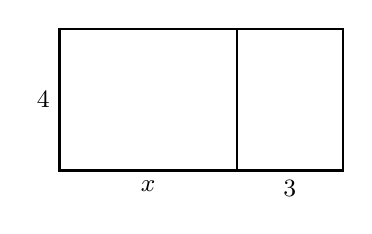
\begin{tikzpicture}[scale=0.45,font=\small]\draw[line width=0.8pt] (0,0) rectangle (8,4);\draw[line width=0.8pt] (5,0) -- (5,4);\node[below] at (2.5,0) {$x$};\node[below] at (6.5,0) {$3$};\node[left] at (0,2.0) {$4$};\end{tikzpicture}\end{minipage}\par\medskip
\noindent\textbf{Aufgaben}\hspace{1em}{\small\color{mbgrau}\karohinweis{C}{Rechne unten im Karo.}{Rechne auf einem extra Blatt.} Vergleiche jede Aufgabe gleich mit dem Lösungsheft.}\par\smallskip
\aufgg{\hangindent7mm\hangafter1\nr{1.}Schreibe einen Term für den Umfang (Maße in cm). \par a)~Quadrat \qquad b)~Rechteck, dazu auch den Flächeninhalt \qquad c)~Dreieck mit drei gleich langen Seiten}{\adjustbox{max width=\linewidth}{\begin{varwidth}{50cm}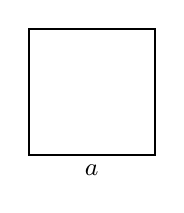
\begin{tikzpicture}[scale=0.4,font=\small]\draw[line width=0.8pt] (0,0) rectangle (4,4);\node[below] at (2.0,0) {$a$};\end{tikzpicture}\qquad 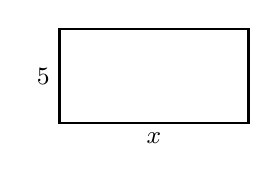
\begin{tikzpicture}[scale=0.4,font=\small]\draw[line width=0.8pt] (0,0) rectangle (6,3);\node[below] at (3.0,0) {$x$};\node[left] at (0,1.5) {$5$};\end{tikzpicture}\qquad 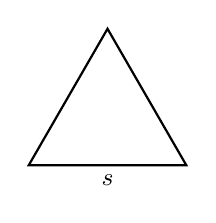
\begin{tikzpicture}[scale=0.4,font=\small]\draw[line width=0.8pt] (0,0) -- (5,0) -- (2.5,4.33) -- cycle;\node[below] at (2.5,0) {$s$};\end{tikzpicture}\end{varwidth}}}{}{}
\medskip
\aufgg{\hangindent7mm\hangafter1\nr{2.}Das Rechteck ist in zwei Streifen geteilt. Welcher Term gibt den Flächeninhalt des ganzen Rechtecks an? Kreuze an.\par\smallskip\leftskip7mm \kreuz{$a \cdot b + c$}\ \kreuz{$a \cdot (b + c)$}\par\kreuz{$a + b \cdot c$}\ \kreuz{$a \cdot b \cdot c$}}{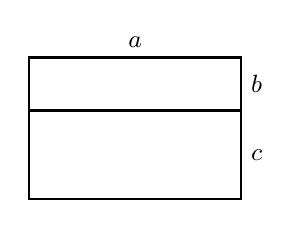
\begin{tikzpicture}[scale=0.45,font=\small]\draw[line width=0.8pt] (0,0) rectangle (6,4.0);\draw[line width=0.8pt] (0,2.5) -- (6,2.5);\node[above] at (3.0,4.0) {$a$};\node[right] at (6,3.25) {$b$};\node[right] at (6,1.25) {$c$};\end{tikzpicture}}{}{}
\medskip
\aufgg{\hangindent7mm\hangafter1\nr{3.}Das Rechteck besteht aus zwei Teilen (Maße in m). \par a)~Schreibe zwei verschiedene Terme für den Flächeninhalt. \par b)~Schreibe einen Term für den Umfang.}{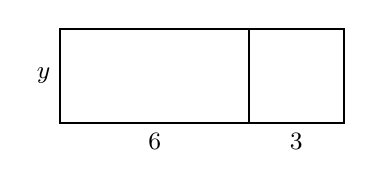
\begin{tikzpicture}[scale=0.4,font=\small]\draw[line width=0.8pt] (0,0) rectangle (9,3);\draw[line width=0.8pt] (6,0) -- (6,3);\node[below] at (3.0,0) {$6$};\node[below] at (7.5,0) {$3$};\node[left] at (0,1.5) {$y$};\end{tikzpicture}}{}{}
\medskip
\aufg{\hangindent7mm\hangafter1\nr{4.}Ein rechteckiges Beet ist $x$ Meter lang und 3 Meter breit. Es bekommt rundherum einen Zaun. \par a)~Skizziere das Beet und schreibe einen Term für die Länge des Zauns. \par b)~Das Beet soll 6 Meter lang werden. Reichen 20 Meter Zaun? \par c)~Wie groß ist dann seine Fläche?}{}{{\scriptsize\color{mbgrau}Ziel\hspace{2mm}}}
\medskip
\par\vspace{3mm}\setlength{\kr}{\dimexpr\pagegoal-\pagetotal-10mm\relax}%
\ifdim\kr>12mm\karomerk{k}{C}\noindent{\scriptsize\color{mbgrau}Platz zum Rechnen}\par\nointerlineskip\vspace{1mm}\noindent
\begin{tikzpicture}\clip (0,0) rectangle ({\linewidth-0.5mm},\kr);\draw[black!16,line width=0.3pt,step=5mm] (0,0) grid (\linewidth,\kr);\end{tikzpicture}\fi\par
\clearpage\label{s:D}\noindent\colorbox{black!12}{\makebox[10mm]{\Large\bfseries\strut D}}\hspace{3mm}{\Large\bfseries Terme in Sachaufgaben}\par\smallskip
\noindent Lege zuerst fest, wofür die Variable steht. Ein fester Betrag wird addiert; was für jedes Stück dazukommt, wird mit der Anzahl malgenommen.\par\medskip
\noindent\textbf{Formel}\par\nopagebreak\noindent\hspace*{4mm}\begin{minipage}{\dimexpr\linewidth-4mm\relax}Preis $=$ fester Betrag $+$ Preis je Stück $\cdot$ Anzahl \quad z.\,B. \ $5 + 2 \cdot x$\end{minipage}\par\medskip
\noindent\textbf{Beispiel}\quad Ein E-Scooter kostet 1 Euro zum Entsperren und 0,20 Euro je Minute. Schreibe einen Term für den Preis einer Fahrt. Was kostet eine Fahrt von 15 Minuten?\par\smallskip
\noindent\par\noindent\hangindent6mm\hangafter1\makebox[6mm][l]{\textbf{1}}Variable festlegen: \ $x$ ist die Zahl der Minuten.\par\smallskip\par\noindent\hangindent6mm\hangafter1\makebox[6mm][l]{\textbf{2}}Fest: 1 Euro. \ Je Minute 0,20 Euro, bei $x$ Minuten: \ $0{,}20 \cdot x$\par\smallskip\par\noindent\hangindent6mm\hangafter1\makebox[6mm][l]{\textbf{3}}Term für den Preis in Euro: \quad $1 + 0{,}20 \cdot x$\par\smallskip\par\noindent\hangindent6mm\hangafter1\makebox[6mm][l]{\textbf{4}}Für 15 Minuten einsetzen: \ $1 + 0{,}20 \cdot 15 = 1 + 3 = 4$. \ Die Fahrt kostet 4 Euro.\par\smallskip\par\medskip
\noindent\textbf{Aufgaben}\hspace{1em}{\small\color{mbgrau}\karohinweis{D}{Rechne unten im Karo.}{Rechne auf einem extra Blatt.} Vergleiche jede Aufgabe gleich mit dem Lösungsheft.}\par\smallskip
\aufg{\hangindent7mm\hangafter1\nr{1.}Beim Bowling zahlt man 4 Euro Schuhmiete und 5 Euro je Spiel. Schreibe einen Term für den Preis bei $n$ Spielen. Was kosten 3 Spiele?}{}{}
\medskip
\aufg{\hangindent7mm\hangafter1\nr{2.}Ein Eis kostet $a$ Euro, ein Getränk $b$ Euro. Familie Kaya kauft 4 Eis und 2 Getränke. \par a)~Schreibe einen Term für den Gesamtpreis. \par b)~Ein Eis kostet 1,50 Euro, ein Getränk 2 Euro. Wie viel zahlt die Familie?}{}{}
\medskip
\aufg{\hangindent7mm\hangafter1\nr{3.}Ein Parkhaus berechnet den Preis in Euro mit dem Term $2 + 1{,}50 \cdot x$. \par a)~Was bedeuten die Zahl 2, die Zahl 1,50 und die Variable $x$? \par b)~Was kosten 4 Stunden?}{}{}
\medskip
\aufg{\hangindent7mm\hangafter1\nr{4.}Kanuverleih Fluss nimmt 10 Euro Grundgebühr und 2 Euro je Stunde. Kanuverleih See nimmt 4 Euro je Stunde ohne Grundgebühr. Familie Roth möchte ein Kanu 6 Stunden leihen. Welcher Verleih ist billiger, und um wie viel?}{}{{\scriptsize\color{mbgrau}Ziel\hspace{2mm}}}
\medskip
\par\vspace{3mm}\setlength{\kr}{\dimexpr\pagegoal-\pagetotal-10mm\relax}%
\ifdim\kr>12mm\karomerk{k}{D}\noindent{\scriptsize\color{mbgrau}Platz zum Rechnen}\par\nointerlineskip\vspace{1mm}\noindent
\begin{tikzpicture}\clip (0,0) rectangle ({\linewidth-0.5mm},\kr);\draw[black!16,line width=0.3pt,step=5mm] (0,0) grid (\linewidth,\kr);\end{tikzpicture}\fi\par
\clearpage\label{s:T}\noindent\colorbox{black!12}{\makebox[10mm]{\Large\bfseries\strut T}}\hspace{3mm}{\Large\bfseries Probetest}\par\smallskip
\noindent Gemischt wie in der Prüfung, ohne Beispiel und ohne Taschenrechner. Etwa 20 Minuten.\par\medskip
\noindent\textbf{Aufgaben}\hspace{1em}{\small\color{mbgrau}\karohinweis{T}{Rechne unten im Karo.}{Rechne auf einem extra Blatt.} Vergleiche jede Aufgabe gleich mit dem Lösungsheft.}\par\smallskip
\aufg{\hangindent7mm\hangafter1\nr{1.}Das Achtfache einer Zahl $x$ wird um 6 vermindert. Kreuze den passenden Term an.\par\smallskip\leftskip7mm \kreuz{$8 \cdot (x - 6)$}\ \kreuz{$6 - 8x$}\par\kreuz{$8x - 6$}\ \kreuz{$8x - 6x$}}{}{}
\medskip
\aufg{\hangindent7mm\hangafter1\nr{2.}Die Summe aus dem Doppelten einer Zahl $x$ und 7 wird halbiert. Kreuze den passenden Term an.\par\smallskip\leftskip7mm \kreuz{$2x + 7 : 2$}\ \kreuz{$(2x + 7) : 2$}\par\kreuz{$2 \cdot (x + 7) : 2$}\ \kreuz{$2x : 7 \cdot 2$}}{}{}
\medskip
\aufgg{\hangindent7mm\hangafter1\nr{3.}Das Rechteck besteht aus zwei Teilen (Maße in cm). Gib einen Term für den Flächeninhalt und einen für den Umfang an.}{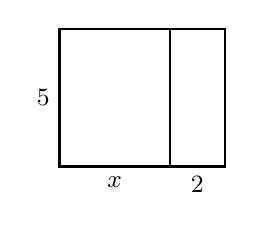
\begin{tikzpicture}[scale=0.35,font=\small]\draw[line width=0.8pt] (0,0) rectangle (6,5);\draw[line width=0.8pt] (4,0) -- (4,5);\node[below] at (2.0,0) {$x$};\node[below] at (5.0,0) {$2$};\node[left] at (0,2.5) {$5$};\end{tikzpicture}}{}{}
\medskip
\aufg{\hangindent7mm\hangafter1\nr{4.}Schreibe als Term: Subtrahiere von einer Zahl $x$ die Zahl 3 und multipliziere die Differenz mit 6.}{}{}
\medskip
\aufg{\hangindent7mm\hangafter1\nr{5.}Ein Bus hat $s$ Sitzplätze und $t$ Stehplätze. Zum Stadion fahren 5 solche Busse. \par a)~Schreibe einen Term für die Zahl der Fahrgäste, die höchstens mitfahren können. \par b)~Wie viele sind es für $s = 40$ und $t = 30$?}{}{}
\medskip
\aufgg{\hangindent7mm\hangafter1\nr{6.}Studio Fit nimmt 20 Euro Aufnahmegebühr und 15 Euro je Monat. Studio Top nimmt 25 Euro je Monat ohne Aufnahmegebühr. \par a)~Schreibe für beide einen Term für die Kosten nach $m$ Monaten. \par b)~Trage die Kosten in die Tabelle ein. \par c)~Ab welchem Monat ist Fit günstiger?}{\adjustbox{max width=\linewidth}{\begin{varwidth}{50cm}\wertetabelle{m}{\text{Fit}}{1,2,3,4,5}\par\wertetabelle{m}{\text{Top}}{1,2,3,4,5}\end{varwidth}}}{}{{\scriptsize\color{mbgrau}Ziel\hspace{2mm}}}
\medskip
\par\vspace{3mm}\setlength{\kr}{\dimexpr\pagegoal-\pagetotal-10mm\relax}%
\ifdim\kr>12mm\karomerk{k}{T}\noindent{\scriptsize\color{mbgrau}Platz zum Rechnen}\par\nointerlineskip\vspace{1mm}\noindent
\begin{tikzpicture}\clip (0,0) rectangle ({\linewidth-0.5mm},\kr);\draw[black!16,line width=0.3pt,step=5mm] (0,0) grid (\linewidth,\kr);\end{tikzpicture}\fi\par
\end{document}
